\documentclass[]{article}

\usepackage{minted}
\usepackage{graphicx}
\usepackage{subcaption}

\usepackage[utf8]{inputenc}
\usepackage[T1]{fontenc}
\usepackage{zlmtt}
\usepackage{fancyvrb}

\usepackage[utf8]{inputenc}
\usepackage{authblk}

\usepackage[a4paper, portrait, margin=1in]{geometry}

\usepackage{natbib}

\setlength{\parindent}{0em}
\setlength{\parskip}{1em}

%opening
\title{Semester Project: Improving the CUDA backend of a domain-specific language compiler in Python}
\author[1]{Langwen Huang}
\author[2]{Supervisor: Eddie Davis}
\author[2]{Oliver Fuhrer}
\affil[1]{Department of Mathematics, ETH Zurich}
\affil[2]{Vulcan Inc.}

\begin{document}

\maketitle

\begin{abstract}
GT4Py is a domain specific language (DSL) for high performance scientific computation by compiling stencil computations into executable codes targeted for various devices including GPUs. It has a prototype \texttt{cuda} backend written in pure Python that provides more flexibility compared to the legacy \texttt{gtcuda} backend. However, the former one is not as optimized as the latter one. This project implemented various optimization techniques including loop reordering, K-loop unrolling, K-caching, prefetching, read-only caching and blocksize adjusting for the \texttt{cuda} backend and benchmarked them using a set of representative stencil computations in GT4Py.
% Result is 10% improvement in some stencils (fillz)
\end{abstract}

\newpage
\tableofcontents
\newpage

\section{Introduction}

\subsection{Computational challenges for weather and climate modeling}
% Need software to improve porting NWC models to CPU/GPU platform
Since the invention of digital computers, weather and climate prediction using numerical models has always been a computational challenge. To achieve more accurate weather and climate predictions, there are continuous efforts of adapting numerical models to the world's largest supercomputers. In recent years, the Moore's law for exponential growth of CPU performance is approaching an end \citep{Theis2017}. This has led many current and emerging supercomputers to hybrid node designs where most of the computational performance is delivered from some form of accelerators such as GPUs. However, this raises the problem of adapting numerical weather and climate models to perform well on such platforms, because the new single-instruction-multiple-thread (SIMT) programming paradigm is required to run efficiently on GPUs, and it is nontrivial to transform the existing source code of numerical models targeted on CPUs into SIMT paradigm.

\cite{Yashiro2016} was the first attempt to adapt the NICAM numerical weather model to GPUs on the TSUNAMI 2.5 supercomputer using OpenACC, followed by \cite{Fu2017} running multiple models on the TaihuLight supercomputer with a similar OpenACC approach and \cite{Bertagna2020} running non-hydrostatic HOMME model on the Summit supercomputer using Kokkos. OpenACC is used for porting existing code to GPU by annotating parallelizable loops in the code while Kokkos allows writing parallel code targeting multiple accelerators including GPUs. Users of OpenACC and Kokkos have to think low level details to make the code efficient. The COSMO-5.0 from MeteoSwiss\citep{Fuhrer2018} is a step forward by decoupling high level numerical code and low level code for the dynamical core using GridTools C++. The LFric model from UK MetOffice takes a similar approach using PSyclone\citep{Adams2019}. Both GridTools and PSyclone are domain specific languages (DSL). Model developers can write in or interpret existing code into such DSLs while experts of supercomputing platforms can optimize DSL compilers. The two combined can make an efficient model running on any supercomputer platforms.

\subsection{GT4Py - a DSL for stencil computation}
% Introduction to GT4Py
%% stencil computation

\begin{figure}[h!]
	\centering
	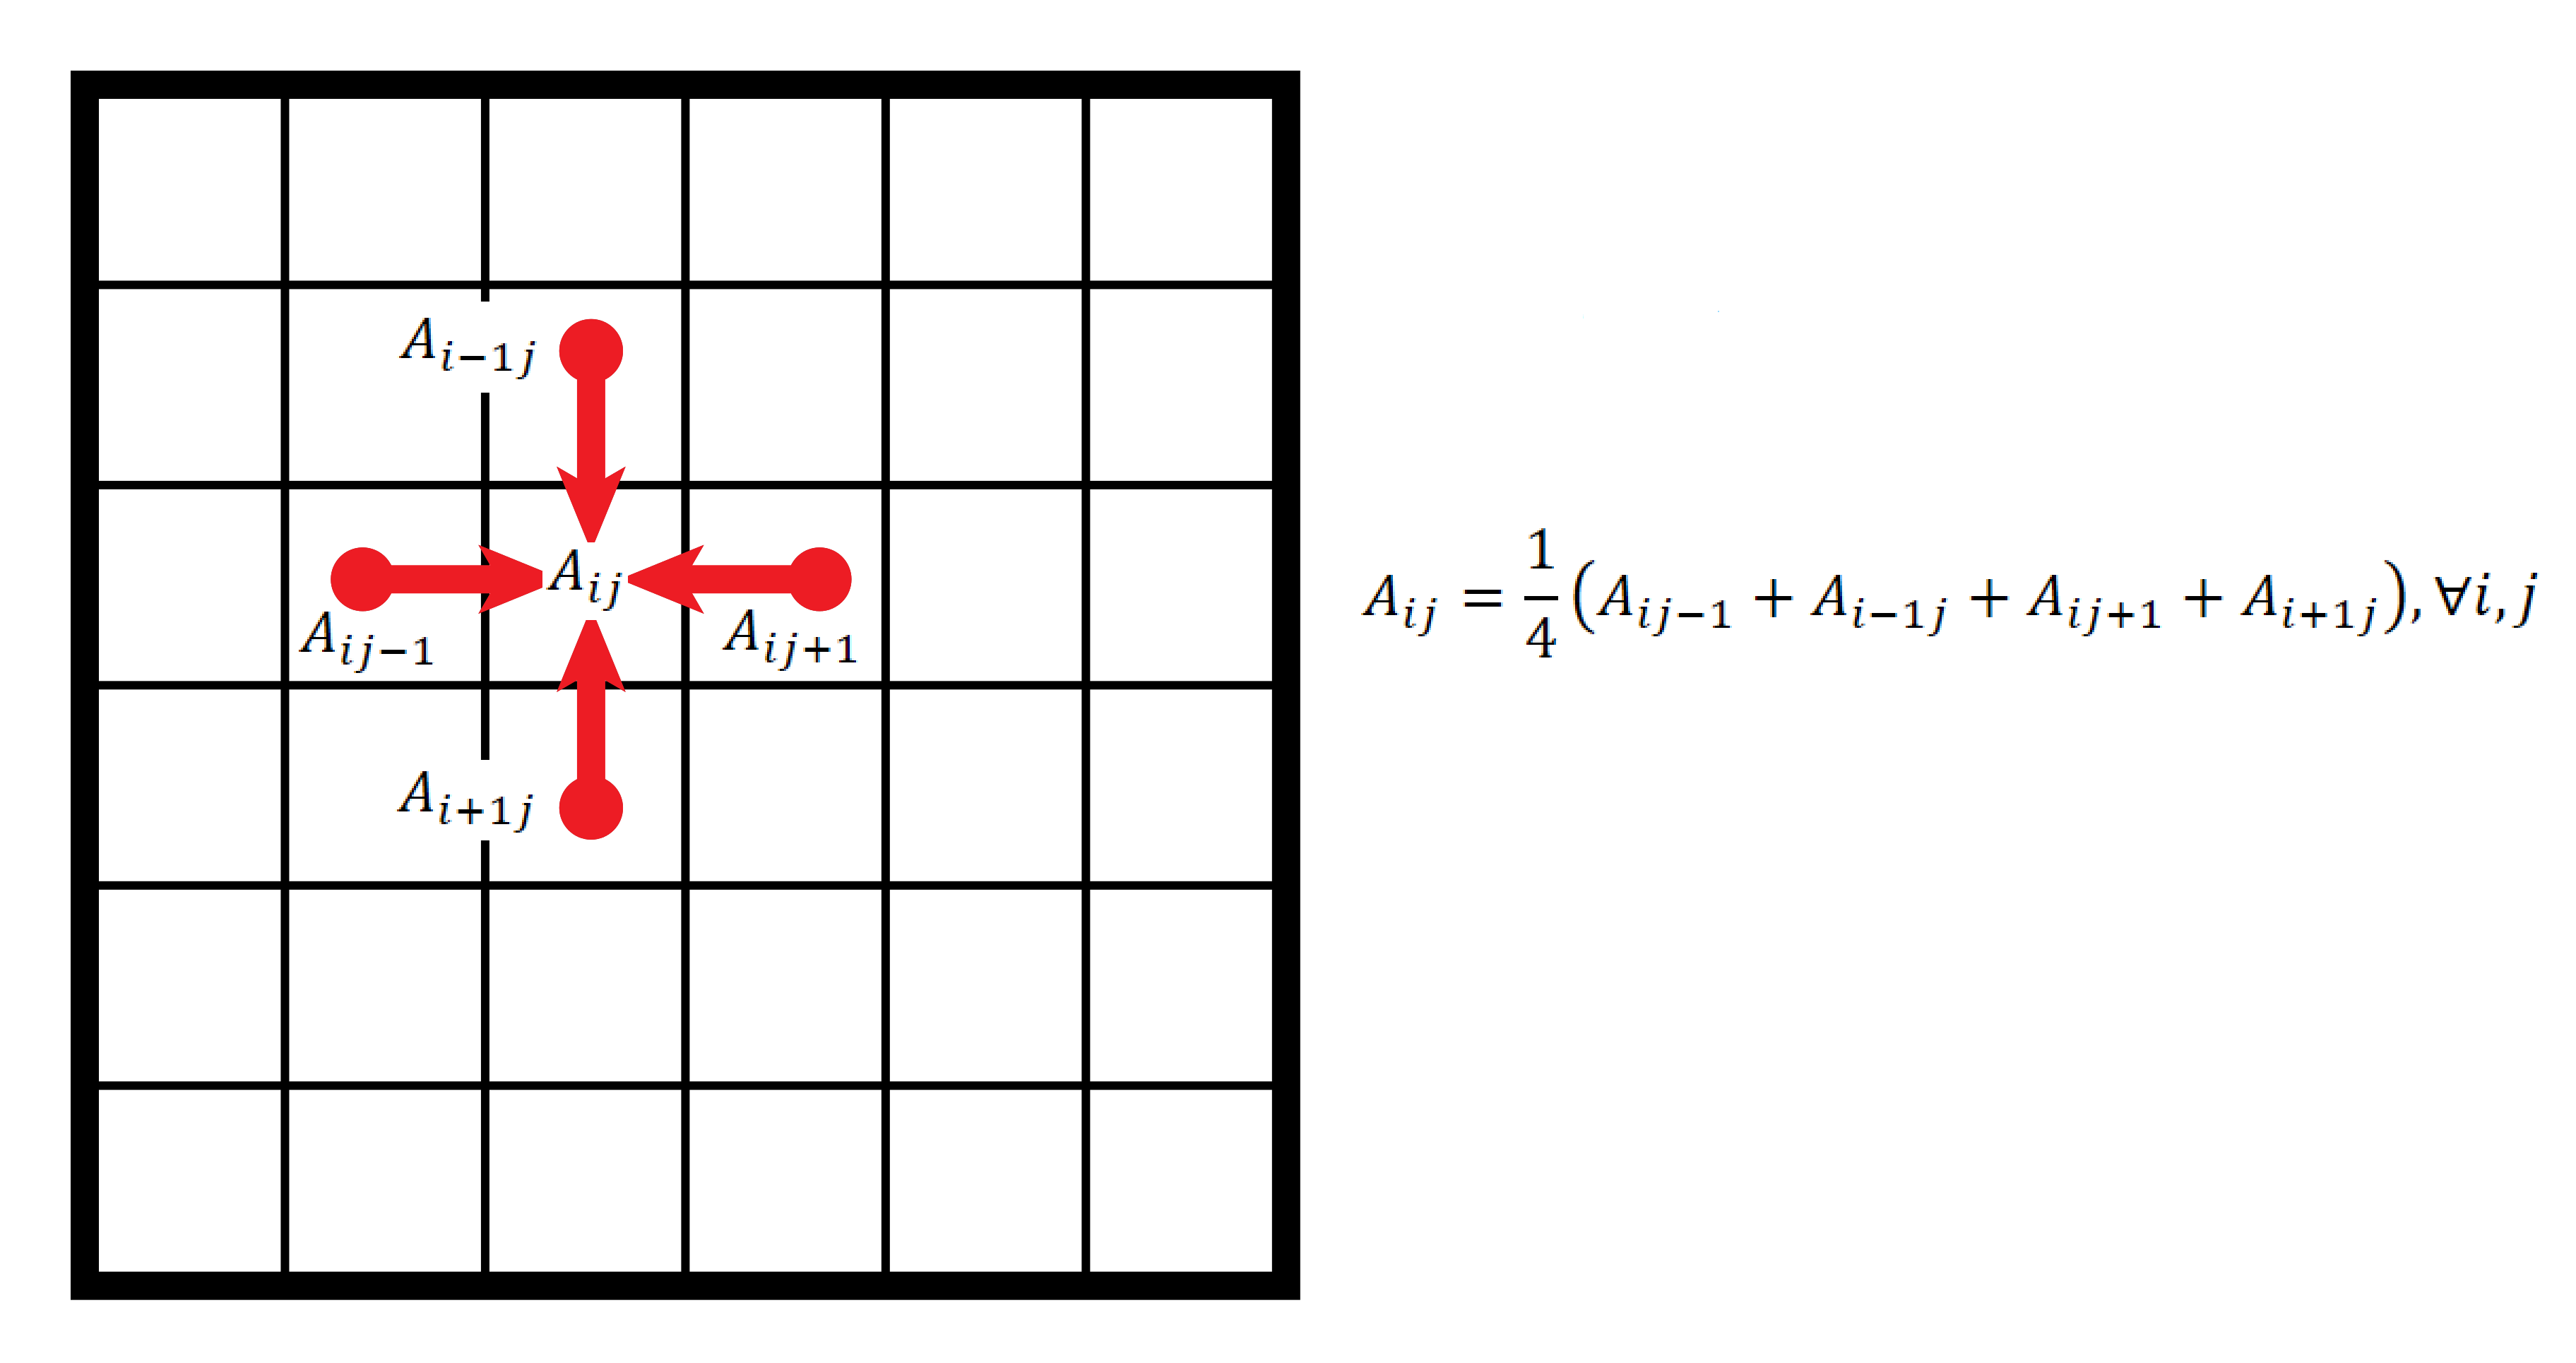
\includegraphics[width=0.7\linewidth]{stencil.png}
	\caption{Diagram of a stencil for Laplacian operator on a 2D grid}\label{fig:stencil}
\end{figure}
Following GridTools C++ and PSyclone's approach, GT4Py is a DSL embeded in the Python language aiming to solve the problem of adapting numerical models to CPU/GPU hybrid platforms. It can interpret stencil computations into low level codes that can execute efficiently on multiple devices including CPU and GPU. A stencil computation represents updating all the values of a field defined on a grid according to the same pattern — called a 'stencil' which is a combination of the surrounding values in the grid. For example, a Laplacian operator applied on a field defined on an infinitely large 2D regular grid can be expressed as a stencil computation, where every value is updated as the average of its upper, lower, left and right neighbors (Figure \ref{fig:stencil}). Most numerical weather and climate models can be expressed as an aggregation of stencil computations, since they are formulated from discretization of the governing partial differential equation (PDE) system, and discretized PDE operator can be easily written as stencil computations like the Laplacian operator.

\subsection{GT4Py internals}
%% (Standard) Compilation process
%% Definition IR -> Implementation IR -> Backend (visitor pattern)
%% Hierarchy: StencilImplementation -> Multistage (Kernel) (api, tempvars) -> group -> stage(accessor) -> applyblock (3D loop)
%% Code snippet from GT4Py code -> pseudo code -> (simplified) CUDA code
% Introduction to GPU, CUDA kernels
%%% https://en.wikibooks.org/wiki/LaTeX/Floats,_Figures_and_Captions
%%% https://tex.stackexchange.com/questions/321750/listing-source-code-in-two-columns/321774
%%% https://tex.stackexchange.com/questions/57353/how-to-get-caption-above-listing-with-minted

GT4Py follows a standard compilation procedure to transform stencils into executable codes: firstly parses the stencil definition into Python AST (Abstract Syntax Tree), then transforms the Python AST into a self defined Definition IR (Intermediate Representation) tree, followed by a series of analysis and optimization passes trying to optimize the underlying computation represented by the IR, and then emits the Implementation IR which is transformed into executable codes by various backends.

There are two backends targeted for GPUs: the \texttt{gtcuda} backend generates GridTools C++ code and uses its GPU backend, the other \texttt{cuda} backend is an experimental backend that directly generates CUDA code. The \texttt{gtcuda} backend provides best performance on platforms with GPUs thanks to the heavily optimized GridTools. However, GridTools is based on C++ templates, which makes it time and memory consuming during compilation, and hard to maintain. The \texttt{cuda} backend frees GT4Py developers from maintaining the obscure C++ template code in GridTools. It is written in pure Python and directly generate human-friendly CUDA code making it much faster and less memory demanding when compiling stencils compared to the \texttt{gtcuda} backend. Additionaly, it is a direct translate of Implementation IR, as a result, the code it generates is less efficient than the \texttt{gtcuda} one.

\begin{minipage}{0.40\linewidth}
\begin{Verbatim}[frame=lines,numbers=left,label=Stencil Definition,framesep=3mm]
@gtscript.stencil()
def thomas_solver_forward(
  a: FIELD_FLOAT,
  b: FIELD_FLOAT,
  c: FIELD_FLOAT,
  d: FIELD_FLOAT,
  x: FIELD_FLOAT):
"""
[b0 c0            ] [x0]   [d0]
[a1 b1 c1         ] [x1]   [d1]
[   a2 b2 c2      ] [x2] = [d2]
[      ...        ] [..]   [..]
[         ... cn-1] [..]   [..]
[            an bn] [xn]   [dn]
"""

  with computation(FORWARD):
    with interval(1, None):
      w = a/b[0, 0, -1]
      b = b - w*c[0, 0, -1]
      d = d - w*d[0, 0, -1]
\end{Verbatim}
\end{minipage}\hfill
\begin{minipage}{0.60\linewidth}
\begin{Verbatim}[frame=lines,label=generated CUDA code,framesep=3mm]
__global__ void multi_stage__31_kernel(
  /* Definition of arguments*/) {
  /* Definition of local variables */
  // stage__16
  for (k=k_min+1+k_block; k<=k_max; k+=k_inc) {
    for (i=i_min+i_block; i<=i_max; i+=i_inc) {
      for (j=j_min+j_block; j<=j_max; j+=j_inc) {
        idx_data_ijk=i*data_strides[0]+
                     j*data_strides[1]+
                     k*data_strides[2];
        idx_data_ijkm1=i*data_strides[0]+
                       j*data_strides[1]+
                       (k-1)*data_strides[2];
        float64_t w;
        w=a[idx_data_ijk]/b[idx_data_ijkm1];
        b[idx_data_ijk]=b[idx_data_ijk]-(w*c[idx_data_ijkm1]);
        d[idx_data_ijk]=d[idx_data_ijk]-(w*d[idx_data_ijkm1]);
      }
    }
  }
}
\end{Verbatim}
\end{minipage}

\subsection{Motivation}
% Comparison of GTCUDA and CUDA backend
%% CUDA backend is slower than GTCUDA
%% Some of the optimization techniques is not available in CUDA backend
%% Like k_cache, ij_cache, loop unrolling

% Reasoning/Motivation for *backend* improvements
%% Motivation
Currently, the dynamical core of the next generation numerical weather model FV3 is being ported to GT4Py by Vulcan Inc. and has been successfully validated to produce the same results as the original one. When running FV3 using GT4Py on platforms with GPUs, the \texttt{cuda} backend is not as performant as the \texttt{gtcuda} backend. However, as \texttt{gtcuda} backend eventually generate CUDA codes as well, there is a potential to improve the performance of the \texttt{cuda} backend. This project aims to design, implement and test different optimization strategies for the \texttt{cuda} backend in order to fullfill such potential.

\section{Method}

\subsection{Benchmark set}
% FV3 core stencils , input data, timing
It is important to quantify the performance of a specific backend before optimizing it. A benchmark set is made choosing the most time consuming stencils from the FV3 project including: \texttt{fillz}, \texttt{sim1\_solver} and \texttt{saturation\_adjustment}. Note that \texttt{sim1\_solver} is called from two Riemann solver stencils \texttt{riem\_solver\_c} and \texttt{riem\_solver3}, we will only benchmark the two instead of \texttt{sim1\_solver} as input data for it is not available. In addition, a Thomas solver (tridiagonal solver) stencil is added to the benchmark set, because it is very common in many numerical weather and climate models.

For input data of FV3 stencils, we use the validation dataset shipped with the FV3-GT4Py project which has appropriate input data for each stencils. We use random data for Thomas solver stencil, and the running time should be the same for any given data since it is a non-oblivious algorithm.

We measure the time of each stencil in the benchmark set running 100 times with a specific GT4Py backend ignoring the time of reading input data. Then the measured times are treated as performance index for the backend to guide adaptation of optimization techniques. All the timings are performed in the \texttt{n1-standard-8} node from Google Cloud with a P100 GPU and 30GB memory, because the ported FV3 usually runs on the supercomputer Piz Daint which has P100 GPU nodes.

\subsection{Optimization techniques}
%% most time consuming stencils are ij independent
%% focus on ij independent optimizations: blocksize adjust, kcaching, ijk loop, kloopunrolling
%% most are memory bound -> improve memory bandwidth/ decrease memory usage
A preliminary profiling to the benchmark set shows that most of the stencils are memory-bound which means we need to find optimization techniques that reduces time of memory operations. Apart from improving specific algorithms which is not possible from a backend's perspective, the general way to reduce memory operations is to utilise the cache hierarchy.
%The mordern GPU architecture maintains a cache hierarchy like CPUs where a cascade of storage devices called caches ranging from fast but low-capacity registers to slow but high-capacity last level cache.
In the definition of stencils, memory accesses only have partial-order meaning that any order satisfying the partial order will produce the same intended result, but the performance of the stencil with different memory access orders may differ because the cache is utilised differently. So, a backend can improve the performance of a memory bound stencil by rearranging memory accesses in a smart way to make efficient use of the cache hierarchy.

Specifically, because the GT4Py is made for 3D stencil computations which allows specifying computation order for the third dimension ("K" dimension or height), we explored possibilites of optimizing memory accesses for the K dimension including loop reordering, K-loop unrolling, K-caching. We also exploited the staticness of stencil computing in the sense of memory access pattern is determined at compile time by using prefetching and read-only caching. In addition, we added an option to vary blocksize configurations to adapt to specific GPU platforms.

%\subsection{Handcrafted optimization for Thomas solver}
% Explore Optimization techniques on Thomas solver
Before implementing optimization techniques into the backend, we made a small CUDA program based on the generated CUDA code of Thomas solver stencil and handcrafted those techniques in the program as a proof of concept. It is also to make sure those techniques are effective or at least not harmful.
% Microbenchmark
% Nsight compute profiling
With the help of Nsight Compute from CUDA Toolkit, we get detailed profile of the program including percentage of computation power and memory bandwidth used, L1/L2 cache hit rate, and wrap stall time. Unfortunately, as Nsight Compute is not compatible with the P100 platform, we performed the profiling on a PC equipped with a NVIDIA RTX 2060 GPU.

\subsubsection{Loop reordering}
% memory layout is C style (x[i,j,k] and x[i+1,j,k] are continuous)
% exploit time-locality
% reduce cache miss for k-dependent loop
% only correct for ij-independent loop
The memory layout of multidimensional array in GT4Py is C-style where \texttt{x[i,j,k]} and \texttt{x[i+1,j,k]} are continuous in memory. The \texttt{cuda} generate stencils into KIJ loops ("I" "J" as first and second dimension) to ensure the correct result when the loop body have offseted memory accesses in both K and IJ directions. But KIJ loops are inefficient for IJ-independent loops where there's only offsets in K direction compared with IJK loops because IJK loops have better time-locality for memory accesses. For example, \texttt{x[i, j, k] = x[i, j, k-1];} requires 1 memory read and 1 memory write in KIJ loops but may only requires 1 cache read and 1 memory write in IJK loops if the cache size is big enough so that \texttt{x[i, j, k]} is not flushed out of the cache.
Therefore, to exploit such time-locality, one would have to identify whether a loop is IJ-independent loop and then swap the loop order.
\begin{Verbatim}[frame=lines,numbers=left,label=Loop reordering,framesep=3mm]
/* Before: */
for (k=k_min+1+k_block; k<=k_max; k+=k_inc)
  for (i=i_min+i_block; i<=i_max; i+=i_inc)
    for (j=j_min+j_block; j<=j_max; j+=j_inc)
      x[i, j, k] = x[i, j, k-1];
/* After loop reordering: */
for (i=i_min+i_block; i<=i_max; i+=i_inc)
  for (j=j_min+j_block; j<=j_max; j+=j_inc)
    for (k=k_min+1+k_block; k<=k_max; k+=k_inc)
      x[i, j, k] = x[i, j, k-1];
\end{Verbatim}
\subsubsection{K-loop unrolling}
% Inherited from gtcuda
% reduce logic operations driving the loop
% allow better reordering of statements for shading memory access
% especially for small loop body
Inspired by GridTools, one can unroll the last level K-loop based on IJK loop optimization to enable the CUDA compiler optimizing redundant memory accesses into register accesses and to give the compiler more flexibility of reordering statements in loop body to hide memory access latency. This technique make use of CUDA compiler using \texttt{\#pragma unroll N} where N is determined in the optimization pass according to number of instructions in the loop body.
\begin{Verbatim}[frame=lines,numbers=left,label=K-loop unrolling,framesep=3mm]
for (i=i_min+i_block; i<=i_max; i+=i_inc)
  for (j=j_min+j_block; j<=j_max; j+=j_inc)
#pragma unroll N // <----K-loop unrolling
    for (k=k_min+1+k_block; k<=k_max; k+=k_inc)
      x[i, j, k] = x[i, j, k-1];
\end{Verbatim}
\subsubsection{K-caching}
% Inherited from gtcuda and dawn compiler
% Can be implemented with shared-memory or local array (register)
% Shared memory is slower than register approach
% k cache of size 2 is sufficient for most case
Also inspired by GridTools and its predecessor the Dawn compiler, K-caching manually inserts cache arrays for memory accesses in along K direction. Since offsets in the K direction are usually $\pm 1$, K cache of size 2 is sufficient for most case. The K-caching technique replaces memory accesses by cache accesses, then inserts cache read at the beginning of the loop body and write-back-to-memory statements at the end if the cache is modified. Also at the end of the loop, the second element of the cache is moved to the first to match the memory position in the next iteration.    
\begin{Verbatim}[frame=lines,numbers=left,label=K-caching,framesep=3mm]
/* Before: */
for (i=i_min+i_block; i<=i_max; i+=i_inc)
  for (j=j_min+j_block; j<=j_max; j+=j_inc)
    for (k=k_min+1+k_block; k<=k_max; k+=k_inc)
      x[i, j, k] = x[i, j, k-1];
/* After K-caching: */
float64_t x_cache[2];
for (i=i_min+i_block; i<=i_max; i+=i_inc)
  for (j=j_min+j_block; j<=j_max; j+=j_inc) {
    x_cache[0] = x[i, j, k_min+k_block];
    for (k=k_min+1+k_block; k<=k_max; k+=k_inc) {
      x_cache[1] = x[i, j, k];
      x_cache[1] = x_cache[0];
      x[i, j, k] = x_cache[1];
      x_cache[0] = x_cache[1];
    }
  }
\end{Verbatim}
\subsubsection{Prefetching}
% As good as shared memory k-caching (shared memory is actually L1 cache)
% reduce cache miss
% Not restricted to ij-independent stencils
Prefetching loads a memory section in to the specific cache before it is used to reduce cache miss which is usually the case for GT4Py stencils. It can be applied to any programs as long as the memory accesses can be predetermined at compile time which is the case for GT4Py. Note that the CUDA language does not officially support prefetching, we use inlined PTX code to insert prefetch instructions. While there are prefetch instructions for both L1 and L2 cache, only L1 prefetching is used because it is more efficient than L2 prefetching when profiling the Thomas solver CUDA program.
\begin{Verbatim}[frame=lines,numbers=left,label=Prefetching,framesep=3mm]
/* Before: */
for (k=k_min+1+k_block; k<=k_max; k+=k_inc)
  for (i=i_min+i_block; i<=i_max; i+=i_inc)
    for (j=j_min+j_block; j<=j_max; j+=j_inc)
      x[i, j, k] = x[i, j, k-1];
/* After prefetching: */
for (k=k_min+1+k_block; k<=k_max; k+=k_inc)
  for (i=i_min+i_block; i<=i_max; i+=i_inc)
    for (j=j_min+j_block; j<=j_max; j+=j_inc)
      prefetch(&x[i, j, k]);
      prefetch(&x[i, j, k-1]);
      x[i, j, k] = x[i, j, k-1];
\end{Verbatim}
\subsubsection{Read-only caching}
% LDG loads persuade GPU to store data in read-only cache
% which has much less latency compared to normal (L1) cache
Similar to prefetching, the read-only caching inserts "load from global memory (LDG)" instructions to memory reads if that memory location is not modified in the CUDA kernel. The LDG instruction persuades GPU to cache the read-only data into read-only cache which has much less latency than normal caches and in turn increase performance.
\begin{Verbatim}[frame=lines,numbers=left,label=Read-only caching,framesep=3mm]
/* Before: */
for (k=k_min+1+k_block; k<=k_max; k+=k_inc)
  for (i=i_min+i_block; i<=i_max; i+=i_inc)
    for (j=j_min+j_block; j<=j_max; j+=j_inc)
      x[i, j, k] = a[i, j, k-1]; // <---- a is read-only
/* After read-only caching: */
for (k=k_min+1+k_block; k<=k_max; k+=k_inc)
  for (i=i_min+i_block; i<=i_max; i+=i_inc)
    for (j=j_min+j_block; j<=j_max; j+=j_inc)
      x[i, j, k] = __ldg(&a[i, j, k-1]);
\end{Verbatim}
\subsubsection{Blocksize adjusting}
% reduce blocksize.y to 1 if it is ij-independent
% search for best blocksize config
% default on gridtools are (256, 8, 1) (new) and (64, 8, 1)
For each memory accesses in 3D loops of \texttt{cuda} generated codes, the GPU accesses a block of data with a predetermined blocksize. The K dimension of the blocksize is always 1 to ensure the correctness of stencil computation with specific K-order requirement, while the blocksizes of IJ dimension can be arbitrary. The \texttt{cuda} backend currently set a constant blocksize of (32, 8, 1), but this may not be the optimal choice as GridTools has default blocksize of (64, 8, 1) or (256, 8, 1) (new version). So we varied the I dimension of the blocksize to find if there is any better choice. Moreover, since GPU read continuous data faster, it makes sense to set the J dimension of the blocksize to one if the stencil only contains IJ-independent loops.

\subsection{Implementation of an optimization pass for \texttt{cuda} backend}
% Implementation (decoupling with backend)
%% Visitor pattern
%% loop <----> applyblock
%% Use/generate Applyblock metadata, edit nodes under Applyblock

% Add diagram of the optimization pass

As an attempt to decouple optimization from backend implementation, we added a new optimization pass between Implementation IR and the \texttt{cuda} backend. The pass follows the visitor pattern, which takes in the root node of the Implementation IR called StencilImplementation node and visit its children node using depth-first search. When it finds nodes of type ApplyBlock representing 3D loops in IR it passes the node to each optimization methods which themselves follow visitor pattern. Each optimization methods either modifies children nodes under the ApplyBlock node mimicking manual insertion/modification of expressions in the loop body, or add metadata to the ApplyBlock node which is identified in the backend to generate code of specific pattern.

The structure of the optimation pass makes it easy to switch on/off any specific optimization technique, so we made a grid search script that benchmarks every combinations of existing techniques to examine the effectiveness of those techniques.
 
\section{Result}
% Roofline model for microbenchmark (or percentage of computation power/memory bandwidth)
\subsection{Profiling result of Thomas solver program}
% Scatter Plot of Mem vs Computation  utilization

% L1 cache is better than L2 cache
% Prefetching is the same as shared memory K-caching
% Register K-caching is better than Prefetching
% Unrolling 2 - 4 loops is effective
% reducing blocksize.y to 1 is effective
%% Nsight not available in P100 -> gridsearch is needed as a final result
 
\subsection{Grid search result}
% Grid search
% Parallel coordinate plot: https://www.data-to-viz.com/graph/parallel.html

%% result vairation -> take the minimum of time?
%% Not much improvements for Sat_adj and Riem_solver3 -> no ij_cache compared to gtcuda?
% Average gain from each optimization method


\section{Conclusion}
% Provide wide range of optimization techniques, can be adapted to various platforms
% using gridsearch
% Proved to be effective on P100 Platform, better than GTCUDA backend (which is used in production)
We presented improvements to the \texttt{cuda} backend as an addition loosely-coupled optimization pass in the backend. The optimization pass implemented loop reordering, K-loop unrolling, K-caching, prefetching, read-only caching and blocksize adjusting.
% Gridsearch of the combination of those techniques shows ...
%The new \texttt{cuda} backend is X% faster in thomas_solver, Y% faster in fillz stencil, ...

% Further Improvement
%% Adaptive optimization method selection based on gridsearching for each stencils in FV3 core
%% ij cache: used for advection operators
%% optimization for temporary variables
We will further look into IJ-caching which might be the reason that the \texttt{cuda} backend is not performing well on stencils that are not IJ-independent. After implenting the IJ-caching, the \texttt{cuda} backend should possess all the backend optimization techniques that \texttt{gtcuda} has.

\section*{Acknowledgement}
The author would like to thank his supervisor Eddie Davis and Oliver Fuhrer and other members in Vulcan Inc. for their kind guidance and inspiring ideas.

\newpage
\bibliographystyle{agsm}
\bibliography{Report}

\end{document}
